%%%%%%%%%%%%%%%%%%%%%%%%%%%%%%%%%%%%%%%%%%%%%%%%%%%%%%%%%%%%%%%%%%%%
%  2026 Summer Proceedings -- chapter contribution
%
%  Siting Clean-Air Shelters for Vulnerability, Not Just Exposure
%  Fatima Asghar
%  NSF REU Site: Computational Modeling Serving Portland
%
%  Built on the official Summer_proceedings_chapter_template.
%  Document class, preamble, section structure, and bibliographystyle
%  match the template exactly -- do not change them.
%
%  HOW TO READ THIS FILE
%  Normal text is drafted and defensible from what exists today.
%  \NEEDS{...} marks something that cannot be written until a number
%  exists, and names exactly which number. Before camera-ready (Aug 23),
%  grep for NEEDS -- the count must be zero.
%%%%%%%%%%%%%%%%%%%%%%%%%%%%%%%%%%%%%%%%%%%%%%%%%%%%%%%%%%%%%%%%%%%%

\documentclass[graybox]{svmult}

\usepackage{type1cm}
\usepackage{makeidx}
\usepackage{graphicx}
\usepackage{multicol}
\usepackage[bottom]{footmisc}
\usepackage{newtxtext}
\usepackage{newtxmath}

% --- additions beyond the template (all safe with svmult) ---
\usepackage{booktabs}
\usepackage{amsmath}
\usepackage{url}
\usepackage{xcolor}       % ONLY for the \NEEDS marker below

% Drafting marker. DELETE this line and all \NEEDS calls before camera-ready.
\newcommand{\NEEDS}[1]{\textcolor{red}{\textbf{[NEEDS: #1]}}}

\makeindex

%%%%%%%%%%%%%%%%%%%%%%%%%%%%%%%%%%%%%%%%%%%%%%%%%%%%%%%%%%%%%%%%%%%%

\begin{document}

\title*{Siting Clean-Air Shelters for Vulnerability, Not Just Exposure:
An Agent-Based Model of Wildfire Smoke and Portland's Unsheltered Residents}
\titlerunning{Siting Clean-Air Shelters for Vulnerability}

\author{Fatima Asghar}

\institute{Fatima Asghar \at Harrisburg Area Community College, Harrisburg, PA,
\email{fxa28196@hawkmail.hacc.edu}}
% NEEDS: confirm this affiliation line. Inferred from your editorial-team email
% domain (hawkmail.hacc.edu). If the REU wants Portland State listed instead,
% or both, change it here.

\maketitle

%%%%%%%%%%%%%%%%%%%%%%%%%%%%%%%%%%%%%%%%%%%%%%%%%%%%%%%%%%%%%%%%%%%%
% Template rule: abstract capped at 200 words. Body below is ~155 words,
% leaving room for the two NEEDS sentences. Recount after filling them in.
%%%%%%%%%%%%%%%%%%%%%%%%%%%%%%%%%%%%%%%%%%%%%%%%%%%%%%%%%%%%%%%%%%%%

\abstract{Emergency clean-air shelters are the main public-health response
available to cities during wildfire smoke events, and unsheltered residents are
the population with no alternative indoor space. Existing siting guidance,
including federal environmental-justice screening tools, treats ambient
PM$_{2.5}$ as producing uniform harm across everyone exposed to it.
Environmental epidemiology has reported for over a decade that PM$_{2.5}$ health
effects are modified by age and by chronic respiratory disease. This chapter asks
whether incorporating that biological heterogeneity changes where shelters should
be placed. I built an agent-based model in Repast Simphony in which simulated
unsheltered residents of Multnomah County, Oregon move on Portland's street
network, decide each hour whether to seek shelter based on local PM$_{2.5}$ and
an individual awareness probability, and accumulate exposure weighted by age- and
comorbidity-specific relative risks. Five placement strategies are compared,
including two full-information benchmarks that target unweighted and
vulnerability-weighted exposure respectively.
\NEEDS{one sentence with the headline result, most likely the spatial divergence index}
\NEEDS{one sentence naming the limitation that most constrains that result}}

%%%%%%%%%%%%%%%%%%%%%%%%%%%%%%%%%%%%%%%%%%%%%%%%%%%%%%%%%%%%%%%%%%%%
\section{Introduction}
\label{sec:1}

Wildfire smoke is becoming a routine summer condition across the western United
States rather than an exceptional event. During the Pacific Northwest smoke
episode of September 7--19, 2020, hourly PM$_{2.5}$ concentrations in Portland,
Oregon exceeded 500~$\mu$g/m$^3$, among the worst urban air-quality readings
recorded anywhere in the world that year. For residents with housing, the
standard public-health advice during such an event is to stay indoors. For people
living unsheltered, that advice has no referent. Emergency clean-air shelters
exist to supply exactly the indoor space this population lacks, which makes the
question of where to put them a direct determinant of who is protected.

The prevailing approach to siting treats exposure as the quantity to minimize:
put capacity where ambient concentrations are highest, or where the most people
are. Federal screening tools such as the EPA's EJScreen, and comparable state
instruments, encode the same premise --- that a given concentration of PM$_{2.5}$
implies a given burden of harm for everyone standing in it.

That premise is not what the epidemiological literature reports. Effect
modification of PM$_{2.5}$-associated cardiorespiratory outcomes by age is well
established in large cohort studies~\cite{di2017}, and modification by
pre-existing respiratory disease has been examined in the time-series literature.
\NEEDS{a properly sourced sentence on comorbidity effect modification --- see
CITATION\_AUDIT.md; this is the claim that currently has no valid citation behind
it} A seventy-year-old with COPD and a thirty-year-old with healthy lungs
standing on the same sidewalk are not experiencing the same
event.\index{effect modification} Whether that difference is large enough to move
a shelter is an empirical question, and it is the one this chapter asks.

I chose this project because the gap between those two framings is unusually
concrete. It is not a dispute about values; it is a testable question about
whether a widely used class of planning tool gives a different answer once you
add information that has been sitting in the health literature for a decade.

The contribution is deliberately two-tailed. I do not claim that vulnerability
weighting produces better shelter placements. I ask whether it produces
\emph{different} ones, and by how much, for a population with the demographic and
clinical profile of Multnomah County's unsheltered residents. If the placements
barely move, that is useful: it means exposure-only tools are adequate here and
practitioners can keep using them. If they move substantially, it means a common
screening approach is systematically mis-siting a scarce resource.

%%%%%%%%%%%%%%%%%%%%%%%%%%%%%%%%%%%%%%%%%%%%%%%%%%%%%%%%%%%%%%%%%%%%
\section{Related Work and Background}
\label{sec:2}

\NEEDS{This section is genuinely unwritten, and it is the cheapest one to finish
because it needs reading, not results. Roughly one page across the three strands
below. The July 1 lecture in the proceedings resource folder covers exactly this.}

Three literatures meet in this project.

\textbf{Facility siting under environmental hazard.} Static index-based
approaches --- gap analysis, accessibility indices, and the screening tools
mentioned in Sect.~\ref{sec:1} --- share an assumption that creating capacity in
a high-need area translates into use of that capacity.
\NEEDS{2--3 citations}

\textbf{Behavioral modeling of disaster mobility.} That assumption fails when
mobility is constrained or risk awareness is uneven, which is the condition this
population is actually in.
\NEEDS{verify and cite the disaster-mobility sources from your proposal ---
Donner \& Rodriguez 2008, Wong et al. 2018}

\textbf{Effect modification of PM$_{2.5}$ health effects.} The stratified
epidemiology that motivates the vulnerability layer~\cite{di2017}.
\NEEDS{this is where the re-sourced asthma and COPD references belong}

The gap this chapter addresses is that the first two literatures and the third
have not been jointly integrated into a shelter-siting framework for unsheltered
populations.

%%%%%%%%%%%%%%%%%%%%%%%%%%%%%%%%%%%%%%%%%%%%%%%%%%%%%%%%%%%%%%%%%%%%
\section{Data and Methodologies}
\label{sec:3}

This section describes the data behind the simulated population and its smoke
exposure (Sect.~\ref{subsec:2}), then the model that moves that population
through the event (Sect.~\ref{subsec:5}).

\subsection{Data Collection}
\label{subsec:2}

\subsubsection{Air quality}

Hourly PM$_{2.5}$ observations for the September 7--19, 2020 event come from EPA
AirNow regulatory monitors within a bounding box covering Multnomah County.
Because monitors are sparse relative to the street network, concentrations at
agent locations are interpolated.
\NEEDS{State plainly whether the runs you report are driven by AirNow
observations or by the synthetic PM$_{2.5}$ profile used during development. If
synthetic, say so in one sentence and describe the profile. This is a legitimate
proof-of-concept choice; the only thing that would be a problem is leaving it
ambiguous.}
\NEEDS{number of monitors, interpolation method, grid resolution}

\subsubsection{Population, shelters, and street network}

The simulated population is synthetic, drawn from aggregate distributions rather
than individual records. Population counts derive from Multnomah County
Point-in-Time data and the HUD Annual Homelessness Assessment
Report~\cite{henry2023}. Shelter locations and capacities come from the
Multnomah County Joint Office of Homeless Services. The street layer is a City of
Portland street shapefile.
\NEEDS{shapefile name, source URL, retrieval date}
\NEEDS{number of agents, number of shelters, number of street nodes}

Age-bin and respiratory-comorbidity prevalences are applied to the synthetic
population from published estimates for people experiencing homelessness.
\NEEDS{name the source, and state whether the estimates are specific to the
unsheltered subgroup or to the general homeless population --- these differ, and
the distinction belongs in the text, not only in a table}

\subsection{Methods}
\label{subsec:5}

\subsubsection{Modeling framework and architecture}

The model is implemented in Repast Simphony~\cite{north2013}, a Java-based
agent-based modeling environment with a built-in geographic projection and an
interactive runtime display.\index{Repast Simphony} Implementation began from
Repast's bundled GIS demonstration model, from which three components were
retained and repurposed: the generic agent class became the unsheltered-resident
agent, the radio-tower class became the shelter, and the demonstration's
water-line geography was replaced with the Portland street layer.

The architecture splits responsibilities across two languages. All preprocessing
--- street-network handling, spatial interpolation of PM$_{2.5}$, sampling of
agent attributes, computation of agent-to-shelter distances, and evaluation of
the placement strategies --- is performed in Python and exported as flat CSV
tables. The Repast layer reads those tables and performs nothing more expensive
than hash lookups. It runs the hourly agent loop and renders the geographic
display. This split keeps every scientific component in a single tested codebase,
and means the simulation contains no routing or interpolation code in Java.

Python preprocessing uses \texttt{pandas} and \texttt{numpy} for tabular work and
\texttt{scipy} for spatial interpolation.
\NEEDS{list the remaining libraries you actually used, with versions}

Large language models were used during this project as follows: Claude
(Anthropic) assisted with code implementation and debugging, with verification of
literature citations and model parameters, and with editing and condensing prose.
\NEEDS{add any other models or tools you used, and correct this description if it
overstates or understates what happened. The template asks for this disclosure
explicitly, and as Editor-in-Chief your disclosure sets the standard the rest of
the volume will be measured against.} All research decisions, model design
choices, and interpretations are my own, and I reviewed and revised all generated
output.

\subsubsection{Agents and the decision rule}

Each agent represents one unsheltered resident, positioned on a street-network
node. Every agent carries three behavioral parameters and two biological ones, as
summarized in Table~\ref{tab:agent-attrs}.

\begin{table}[ht]
\caption{Attributes carried by each simulated resident.}
\label{tab:agent-attrs}
\begin{tabular}{p{3.4cm}p{7.2cm}}
\hline\noalign{\smallskip}
Attribute & Description \\
\noalign{\smallskip}\svhline\noalign{\smallskip}
Awareness probability & Per-hour probability the agent perceives that air quality
warrants seeking shelter \\
Maximum travel distance & Farthest the agent will travel to reach a shelter \\
Exposure sensitivity & Scalar on realized exposure, representing variation in
time spent outdoors \\
Age bin & One of under-18, 18--44, 45--64, 65+ \\
Comorbidity & One of none, asthma, COPD \\
\noalign{\smallskip}\hline\noalign{\smallskip}
\end{tabular}
\end{table}

At each simulated hour, an agent observes the PM$_{2.5}$ concentration at its
current node. Two transitions are possible. If the agent is not sheltered, local
PM$_{2.5}$ exceeds the EPA ``Unhealthy for Sensitive Groups'' threshold of
35.4~$\mu$g/m$^3$, and a Bernoulli draw against its awareness probability
succeeds, the agent moves to the nearest shelter within its travel distance that
has remaining capacity; shelters at capacity are skipped, so occupancy is
bounded. If the agent is sheltered and local PM$_{2.5}$ has fallen to or below
the threshold, it returns to its origin node.

The return-home rule matters for strategy comparison. Without it, shelter
occupancy rises monotonically across the event and every strategy converges
toward whichever shelters agents happened to reach first, which confounds the
comparison this chapter exists to make.

Sheltered agents accumulate exposure at the outdoor concentration multiplied by
an indoor/outdoor filtration factor.
\NEEDS{state the filtration value used and cite it --- the value in the
implementation guide is attributed to a source that has not been verified, and it
multiplies every sheltered agent-hour in the model}

\subsubsection{The vulnerability-weighted exposure metric}

The central quantity is vulnerability-weighted exposure (VWE), accumulated per
agent per hour:

\begin{equation}
\mathrm{VWE} = \mathrm{PM}_{2.5} \times \mathrm{RR}_{\mathrm{age}} \times
\mathrm{RR}_{\mathrm{comorbidity}}
\label{eq:vwe}
\end{equation}

\NEEDS{THE RELATIVE-RISK TABLE GOES HERE AND CANNOT BE WRITTEN YET. See
CITATION\_AUDIT.md. The asthma, COPD, and under-18 values currently in the
implementation guide are attributed to papers that do not report them. Each RR
needs a source that actually reports PM$_{2.5}$ effect modification for that
stratum, with the effect estimate, 95\% CI, exposure metric (per 10
$\mu$g/m$^3$? per IQR?), and outcome. Highest-priority item before Aug 23.}

Equation~\ref{eq:vwe} combines the two multipliers multiplicatively, which
assumes the age and comorbidity effects are independent. That independence has
not been established in the literature, and it is stated here as an explicit
modeling assumption rather than a finding.
\NEEDS{report the additive-combination sensitivity analysis, or state that it was
not run}

\subsubsection{Placement strategies}

Five strategies are compared, holding the number of shelters fixed. \emph{Status
quo} uses the existing shelter locations. \emph{Density} places shelters at the
nodes of highest agent density. \emph{Gap index} places them at high-population
nodes least well served by existing capacity. The two \emph{oracles} are
full-information benchmarks: the PM$_{2.5}$ oracle places shelters to relieve the
greatest total unweighted exposure within their catchment, and the VWE oracle
does the same for vulnerability-weighted exposure.

Both oracles are greedy catchment-coverage approximations, not exact
optimizations. They provide an upper reference line rather than a solution to the
underlying facility-location problem, and the gap between greedy and exact is not
characterized here.

\subsubsection{Outcome measures}

Runs are scored on total exposure-hours above 35.4~$\mu$g/m$^3$; mean cumulative
PM$_{2.5}$ and mean cumulative VWE per agent; the Gini coefficient of cumulative
exposure across agents, and of VWE; and the \emph{spatial divergence index}, the
fraction of candidate locations where the PM$_{2.5}$ oracle and the VWE oracle
disagree on top-quintile priority. The divergence index is the headline quantity:
it measures directly how much vulnerability weighting moves the answer, and both
a large and a small value are interpretable results.

%%%%%%%%%%%%%%%%%%%%%%%%%%%%%%%%%%%%%%%%%%%%%%%%%%%%%%%%%%%%%%%%%%%%
\section{Results}
\label{sec:4}

\NEEDS{THIS ENTIRE SECTION requires simulation runs. The structure below is
ready; each subsection names the number it needs. Fill top to bottom as runs
land.}

\subsubsection{Model verification}

Before any strategy comparison, the agent logic was checked against cases whose
answers can be worked out by hand.
\NEEDS{Report four small tests as a short table: (a) an agent below threshold
never moves; (b) an agent above threshold with awareness 1.0 and a shelter in
range always moves; (c) a capacity-1 shelter never holds two agents; (d) agents
return home when concentration falls. Give the observed value for each. This
subsection is writable as soon as the model runs at all, and it is what makes the
rest of the section credible.}

\subsubsection{Baseline exposure under the status quo}

\NEEDS{mean cumulative PM$_{2.5}$ per agent, mean VWE, exposure-hours above
threshold, Gini. Plus the run configuration: number of agents, hours simulated,
number of shelters, random seed.}

\subsubsection{Strategy comparison}

\NEEDS{Table 2, the core of the chapter: five strategies as rows; mean
PM$_{2.5}$, mean VWE, exposure-hours, Gini(PM$_{2.5}$), Gini(VWE) as columns.}

\subsubsection{Spatial divergence between the two oracles}

\NEEDS{The most important number in the chapter: the fraction of top-quintile
priority locations where the two oracles disagree, reported under each mobility
assumption.}

\subsubsection{Sensitivity}

\NEEDS{How strategy rankings respond to the three behavioral parameters across
their swept ranges, and to comorbidity prevalence. State the pre-registered
prediction --- that gap-index and density converge under low mobility --- and
whether it held. That prediction is a calibration check on the behavioral layer,
so a failure would be informative rather than merely negative.}

% ------------------------------------------------------------------
% FIGURE PLAN
% Proceedings guidance: EPS wherever possible, from a vector tool
% (matplotlib for plots, Inkscape for drawn figures). PNG/JPG only for photos.
% From matplotlib:
%   fig.savefig("fig1.eps", format="eps", bbox_inches="tight")
%
%   fig1  Model schematic: Python preprocessing -> CSV -> Repast loop ->
%         outputs. Vector, drawn in Inkscape. WRITABLE NOW, no results needed.
%   fig2  Study area: street network, shelter locations, agent starting
%         positions. Matplotlib. WRITABLE NOW.
%   fig3  Exposure accumulation over the event, status quo vs. VWE oracle.
%         Needs runs.
%   fig4  Strategy comparison: mean VWE by strategy, grouped by mobility
%         assumption. Needs the sweep.
%   fig5  Divergence map: locations where the two oracles disagree. Needs runs.
%         This is the money figure -- it shows the finding instead of stating it.
%   fig6  Lorenz curves / Gini by strategy. Optional.
%
% Template's include line omits the file extension so LaTeX picks the format:
%   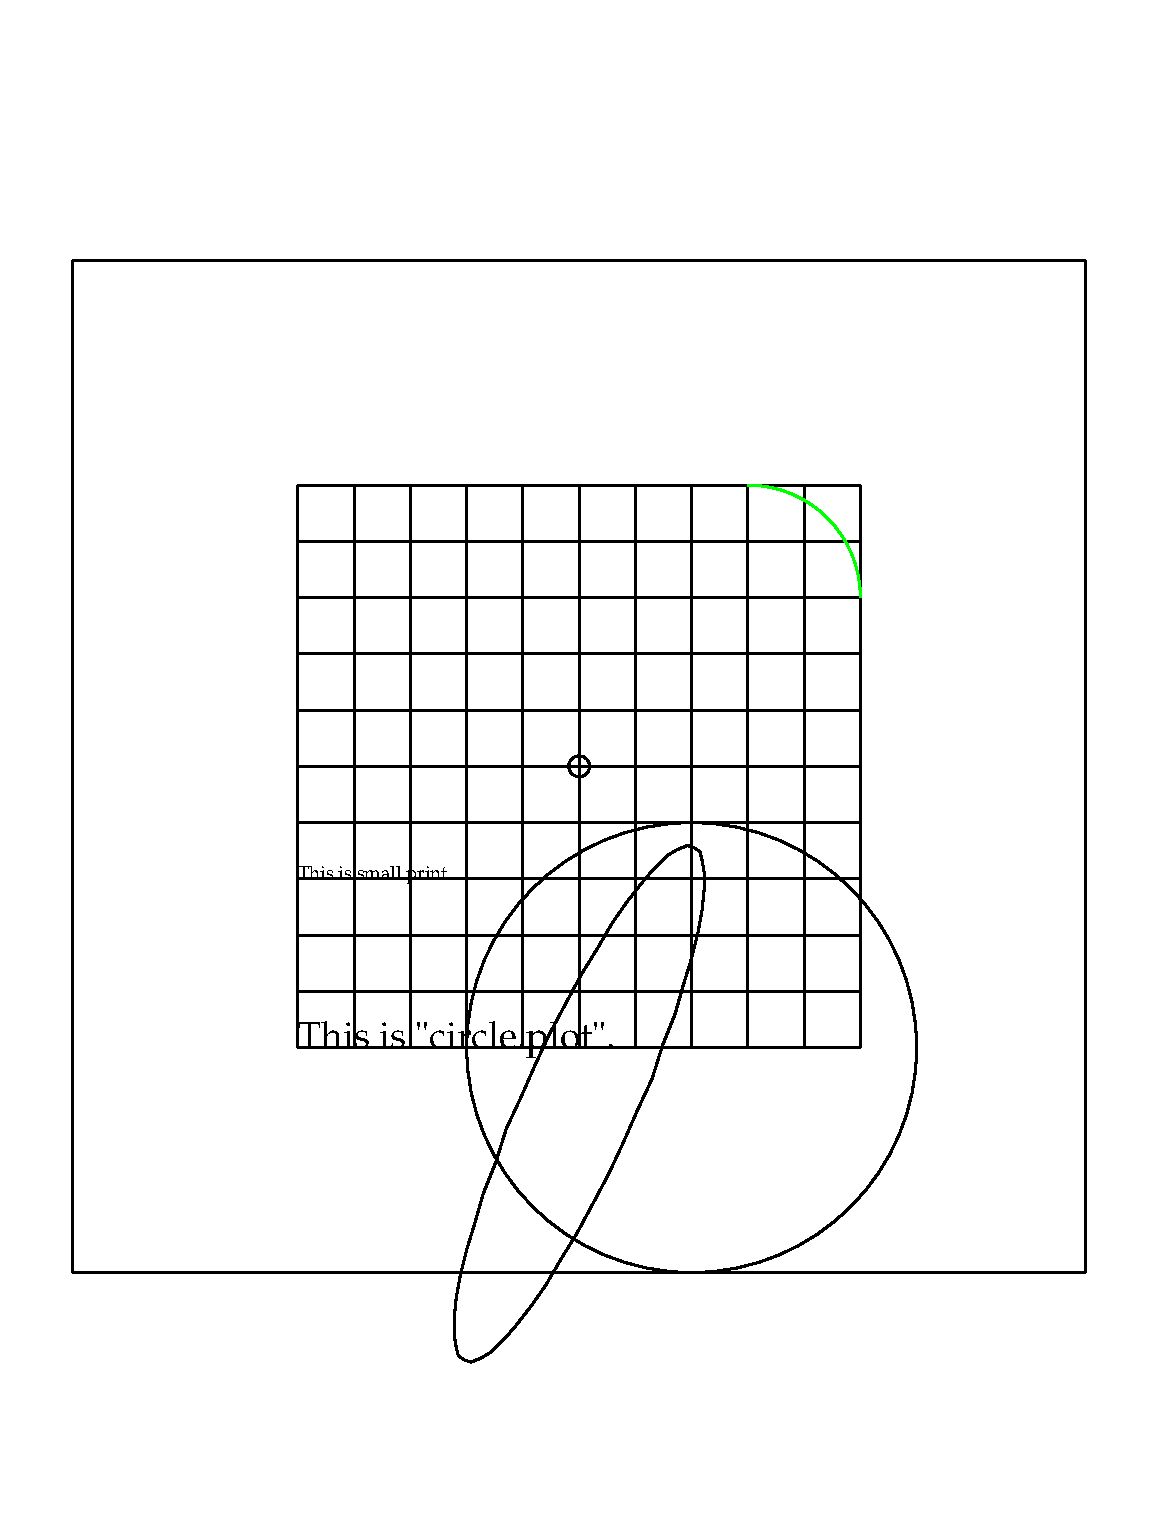
\includegraphics[width=.7\textwidth]{figure}
% ------------------------------------------------------------------

\begin{figure}[ht]
  \centering
  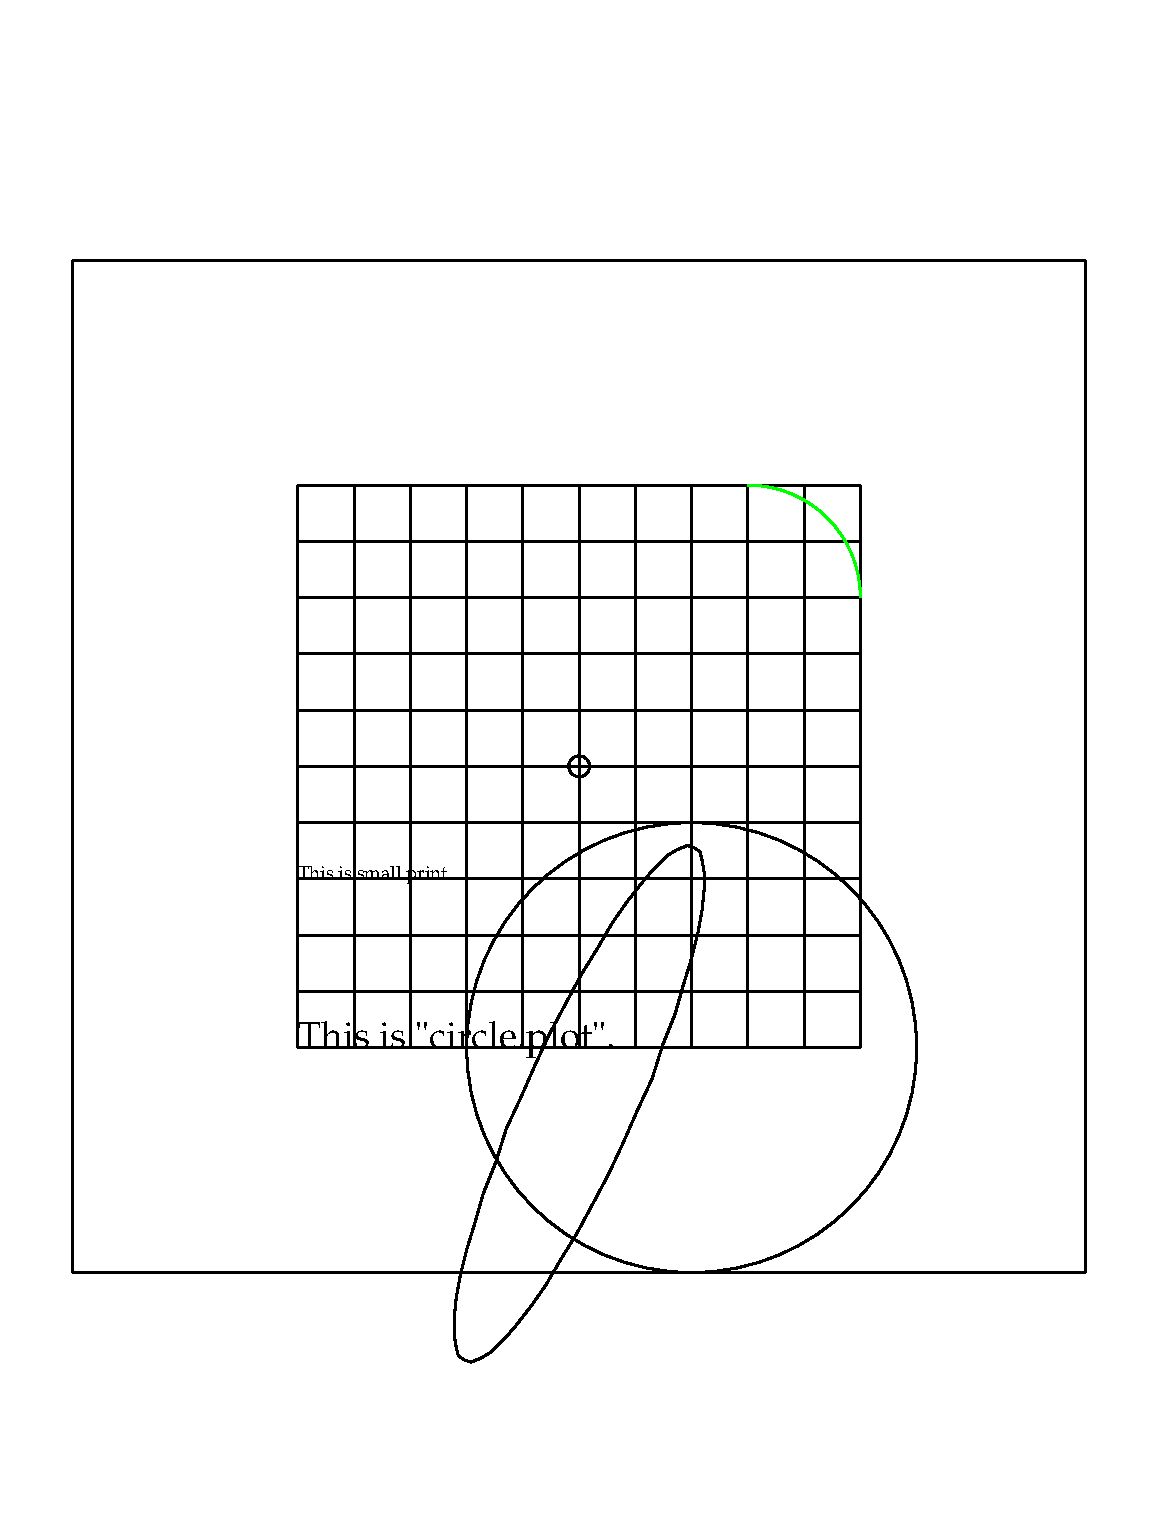
\includegraphics[width=.7\textwidth]{figure}
  \caption{\NEEDS{Replace the placeholder with fig1 (model schematic), and write
  a caption stating what the reader should take away, not just what is shown.}}
  \label{fig:1}
\end{figure}

%%%%%%%%%%%%%%%%%%%%%%%%%%%%%%%%%%%%%%%%%%%%%%%%%%%%%%%%%%%%%%%%%%%%
\section{Conclusion}
\label{sec:5}

\subsection{Applications}

\NEEDS{Two or three paragraphs once results exist. The framing to aim for: this
is a screening tool for a planning question, not a prediction of what would
happen in a specific future event. Name who could use it --- the Multnomah County
Homeless Services Department and Street Roots are both in your proposal --- and
what decision it would inform. If the divergence index turns out small, the
application is still real: it tells planners that simpler exposure-based tools
are sufficient here, which saves them effort.}

\subsection{Concerns and Next Steps}

The limitations below constrain what this chapter can claim.

\begin{itemize}

\item \textbf{Relative-risk provenance.} \NEEDS{State plainly whatever state the
RR sourcing ends in. If a value remains weakly sourced, say so, and report how
sensitive the conclusion is to it. A limitation you name is scholarship; a
limitation you hide is a problem.}

\item \textbf{Multiplicative independence.} Equation~\ref{eq:vwe} assumes the age
and comorbidity effects combine independently. This is untested in the
literature.

\item \textbf{Synthetic population.} Agents are drawn from aggregate
distributions, not individual records. The model speaks to population-level
patterns and cannot speak to any individual.

\item \textbf{Behavioral parameters are assumed, not measured.} No empirical
observations of unsheltered residents' movement during smoke events inform the
awareness or travel-distance values. Results are therefore conditional on
mobility assumptions rather than absolute.

\item \textbf{Greedy oracles.} Both benchmarks are approximations and provide
upper reference lines, not optimal placements.

\item \textbf{No external validation.} \NEEDS{State directly if the county-level
comparison against Oregon Health Authority respiratory data was not run.
Deferring it is a legitimate scope decision for a ten-week project; unvalidated
results simply have to be labeled unvalidated.}

\item \NEEDS{scale --- number of agents and hours simulated, and what that limits}

\end{itemize}

\NEEDS{Close with next steps: real AirNow data if the reported runs used
synthetic PM$_{2.5}$; external validation; exact rather than greedy optimization;
projected-future scenarios; the fall replication.}

%%%%%%%%%%%%%%%%%%%%%%%%%%%%%%%%%%%%%%%%%%%%%%%%%%%%%%%%%%%%%%%%%%%%
\begin{acknowledgement}
This work was completed through the National Science Foundation Research
Experiences for Undergraduates program, Computational Modeling Serving Portland,
hosted by Portland State University. I thank Christof Teuscher for his mentorship
and guidance throughout the program.
\NEEDS{acknowledge anyone else --- other mentors, community partners, anyone who
shared data or gave feedback}

I directed the research, made all research decisions, and wrote the manuscript.
Use of large language models is described in Sect.~\ref{subsec:5}. I reviewed,
revised, and approved all outputs and take full responsibility for the final
text.
\end{acknowledgement}

%%%%%%%%%%%%%%%%%%%%%%%%%%%%%%%%%%%%%%%%%%%%%%%%%%%%%%%%%%%%%%%%%%%%
\noindent\textbf{Code availability.}
\NEEDS{repository URL, and the Zenodo DOI once minted. State the fixed random
seed used for the reported results, so someone can reproduce them.}

% Bibliography -- order and style match the template exactly
\bibliography{references}
\bibliographystyle{plain}

\end{document}
